
\documentclass[a4 paper,12pt]{article}
\usepackage[inner=2.0cm,outer=2.0cm,top=2.5cm,bottom=2.5cm]{geometry}
\usepackage{setspace}
\usepackage{appendix}
\usepackage[rgb]{xcolor}
\usepackage{tabu}
\usepackage{multirow}
\usepackage{longtable}
\usepackage{graphicx}
\usepackage{verbatim}
\usepackage{longtable}
\usepackage{subcaption}
\usepackage{fancyhdr}
\usepackage[colorlinks=true, urlcolor=blue, linkcolor=blue, citecolor=blue]{hyperref}
\usepackage{booktabs}
\usepackage{amsmath,amsfonts,amsthm,amssymb}
\usepackage{setspace}
\usepackage{fancyhdr}
\usepackage{lastpage}
\usepackage{tikz}
\usepackage{listings}
%\lstset{
	%	commentstyle=\color{red!50!green!50!blue!50},%代码块背景色为浅灰色
	%	rulesepcolor= \color{gray}, %代码块边框颜色
	%	breaklines=true,  %代码过长则换行
	%	numbers=left, %行号在左侧显示
	%	numberstyle= \small,%行号字体
	%	keywordstyle= \color{blue},%关键字颜色
	%	frame=shadowbox,%用方框框住代码块
	%	basicstyle=\ttfamily
	%}
\definecolor{dkgreen}{rgb}{0,0.6,0}
\definecolor{mauve}{rgb}{0.9,0.1,0.4}
\definecolor{ash}{rgb}{0.8,0.8,0.8}
\lstset{ 
	language=Octave,                % the language of the code
	basicstyle=\ttfamily,           % the size of the fonts that are used for the code
	numbers=left,                   % where to put the line-numbers
	numberstyle=\small\color{gray},  % the style that is used for the line-numbers
	stepnumber=2,                   % the step between two line-numbers. If it's 1, each line
	% will be numbered
	numbersep=5pt,                  % how far the line-numbers are from the code
	backgroundcolor=\color{ash},      % choose the background color. You must add \usepackage{color}
	rulesepcolor= \color{gray}, %代码块边框颜色
	showspaces=false,               % show spaces adding particular underscores
	showstringspaces=false,         % underline spaces within strings
	showtabs=false,                 % show tabs within strings adding particular underscores
	frame=single,                   % adds a frame around the code
	rulecolor=\color{black},        % if not set, the frame-color may be changed on line-breaks within not-black text (e.g. commens (green here))
	tabsize=2,                      % sets default tabsize to 2 spaces
	captionpos=b,                   % sets the caption-position to bottom
	breaklines=true,                % sets automatic line breaking
	breakatwhitespace=false,        % sets if automatic breaks should only happen at whitespace
	title=\lstname,                   % show the filename of files included with \lstinputlisting;
	% also try caption instead of title
	frame=shadowbox,%用方框框住代码块
	keywordstyle=\color{blue},          % keyword style
	commentstyle=\color{dkgreen},       % comment style
	stringstyle=\color{mauve},         % string literal style
	escapeinside={\%*}{*)},            % if you want to add LaTeX within your code
	morekeywords={*,...}               % if you want to add more keywords to the set
}
\usetikzlibrary{positioning, arrows.meta}
\usepackage{extramarks}
\usepackage{ctex,amsmath,amsfonts,amssymb,bm,hyperref,graphicx}
\usepackage{chngpage}
\usepackage{soul,color}
\usepackage{graphicx,float,wrapfig}
\newcommand{\homework}[3]{
	\pagestyle{myheadings}
	\thispagestyle{plain}
	\newpage
	\setcounter{page}{1}
	\noindent
	\begin{center}
		\framebox{
			\vbox{\vspace{2mm}
				\hbox to 6.28in { {\bf 现代电子电路基础及实验报告 \hfill} {\hfill {\rm #2} {\rm #3}} }
				\vspace{4mm}
				\hbox to 6.28in { {\Large \hfill #1  \hfill} }
				\vspace{3mm}}
		}
	\end{center}
	\vspace*{4mm}
}
\newcommand\numberthis{\addtocounter{equation}{1}\tag{\theequation}}

\begin{document}
	\homework{放大器的频率特性研究实验}{1900011413}{吴熙楠}
	
	\section{实验目的}
	(1)研究放大器的频率特性;
	\par (2) 练习信号源、示波器的使用。
	\section{实验器材}
	直流稳压电源、示波器、信号发生器、放大器实验板。
	\section{实验原理}
	放大器所放大的信号往往是包含许多频率成分的信号,由于放大器特别是交流放大电路中含有耦合电容、旁路电容、分布电容及晶体管极间电容等,使放大倍数与信号的频率有关,这种关系称为放大器的频率特性,放大倍数的幅度与频率的关系称为放大器的幅频特性。
	\par 在一个较宽的频率范围内,曲线是平坦的,即放大倍数是相等的,这段频率范围称为放大器的中频段,放大倍数记做$A_{um}$,随着频率的升高和降低,当放大倍数下降到中频放大倍数的$\frac{1}{\sqrt{2}}$时,所对应的低频和高频截止频率,分别称为放大器的下界频率$f_{L}$和上界频率$f_{H}$。在$f_{L}$和$f_{H}$之间的频率范围内,放大器几乎有相同的放大能力,这一频率范围称为放大器的通频带,以$BW$表示,即$BW=f_{H}-f_{L}$。
	\par 1.单极放大器的低频特性,在低频段,耦合电容和旁路电容不能忽略,它可近似等效为一个高通电路。
	\par 2.单极放大器的高频特性,在高频段,耦合电容的影响可以忽略,但与有关电阻并联的电容、晶体管极间电容和分布电容所造成的影响就必须考虑了。
    \section{实验内容(测量单级放大器的幅频特性)}
    		\begin{figure}[H]
    	\centering
    	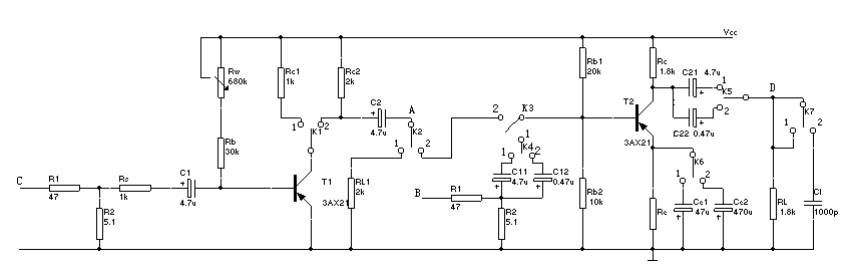
\includegraphics[width=10cm,height=4cm]  {电路板.png} 
    	\caption{\label{1} 实验用电路示意图}
    	\end{figure}
    先将$T_{1}$放大器脱开,只测量实验板右边放大器。将开关$K_{3}、K_{4}、K_{5}、K_{6}、K_{7}$均合向“1”位置,即为测量电路右侧单级放大器。元件参数取 $C_{1}=C_{11}=4.7\mu F,C_{2}=C_{21}=4.7\mu F,C_{e}=C_{e1}=47\mu F,C_{L}$不接入电路。B 点对地输入频率为5kHz 的正弦信号,$u_{s}=200-300mV_{p-p}$。用示波器监视放大器输入信号$u_{i}$,调节信号发生器使放大器输入信号有效值$u_{i}=10mV_{rms}$。用示波器监测放大器的 D 点输出电压,用逐点法测量放大器的幅频特性。
    \par 然后保持放大器输入电压不变,从 5kHz 分别向低端和高端改变放大器输入信号的频率。选择一些
    有代表性的频率,用示波器自动或手动测量并记录该频率及放大器输出电压的相对幅度。由此,即可作出放大器的电压放大倍数随频率变化的曲线,并求出放大器通频带的高、低频截止频率$f_{H},f_{L}$,计算出此时放大器中频段的放大倍数$A_{2}$。

    \section{实验数据处理}
    \subsection{开关全合向“1”位置}
    \begin{table}[H]
    	\centering
    	\caption{实验一数据表($u_{i}=0.252V$)}
    	\label{实验一数据表}
    	\begin{tabular}{|r|r|r|r|r|r|r|r|r|r|r|r|}
    		\toprule[0.5mm]
    		$Hz$&50&100&200&290&300&310&320&330&340&350&360\\
    		$u_{s}/V$&0.22&0.38&0.70&0.86&0.88&0.88&0.88&0.90&0.92&0.94&0.94\\
    		\midrule
    		$Hz$&370&380&390&400&450&500&600&700&800&1k&2k\\
    		$u_{s}/V$&0.96&0.96&0.96&0.98&1.00&1.04&1.08&1.10&1.12&1.14&1.18\\
    		\midrule
    		$Hz$&3k&4k&5k&10k&15k&20k&25k&30k&35k&40k&45k\\
    		$u_{s}/V$&1.22&1.22&1.22&1.22&1.22&1.20&1.18&1.18&1.14&1.14&1.12\\
    		\midrule
    		$Hz$&50k&60k&70k&80k&90k&95k&100k&200k&300k&400k&500k\\
    		$u_{s}/V$&1.10&1.06&1.02&0.98&0.94&0.90&0.86&0.58&0.42&0.30&0.26\\
    		\bottomrule[0.5mm]
    	\end{tabular}
    \end{table}
\par 我们可以从上表得出$f_{H}=100kHz,f_{L}=290Hz,BW\approx 100kHz,A_{2}\approx 4.84$。
		\begin{figure}[H]
	\centering
	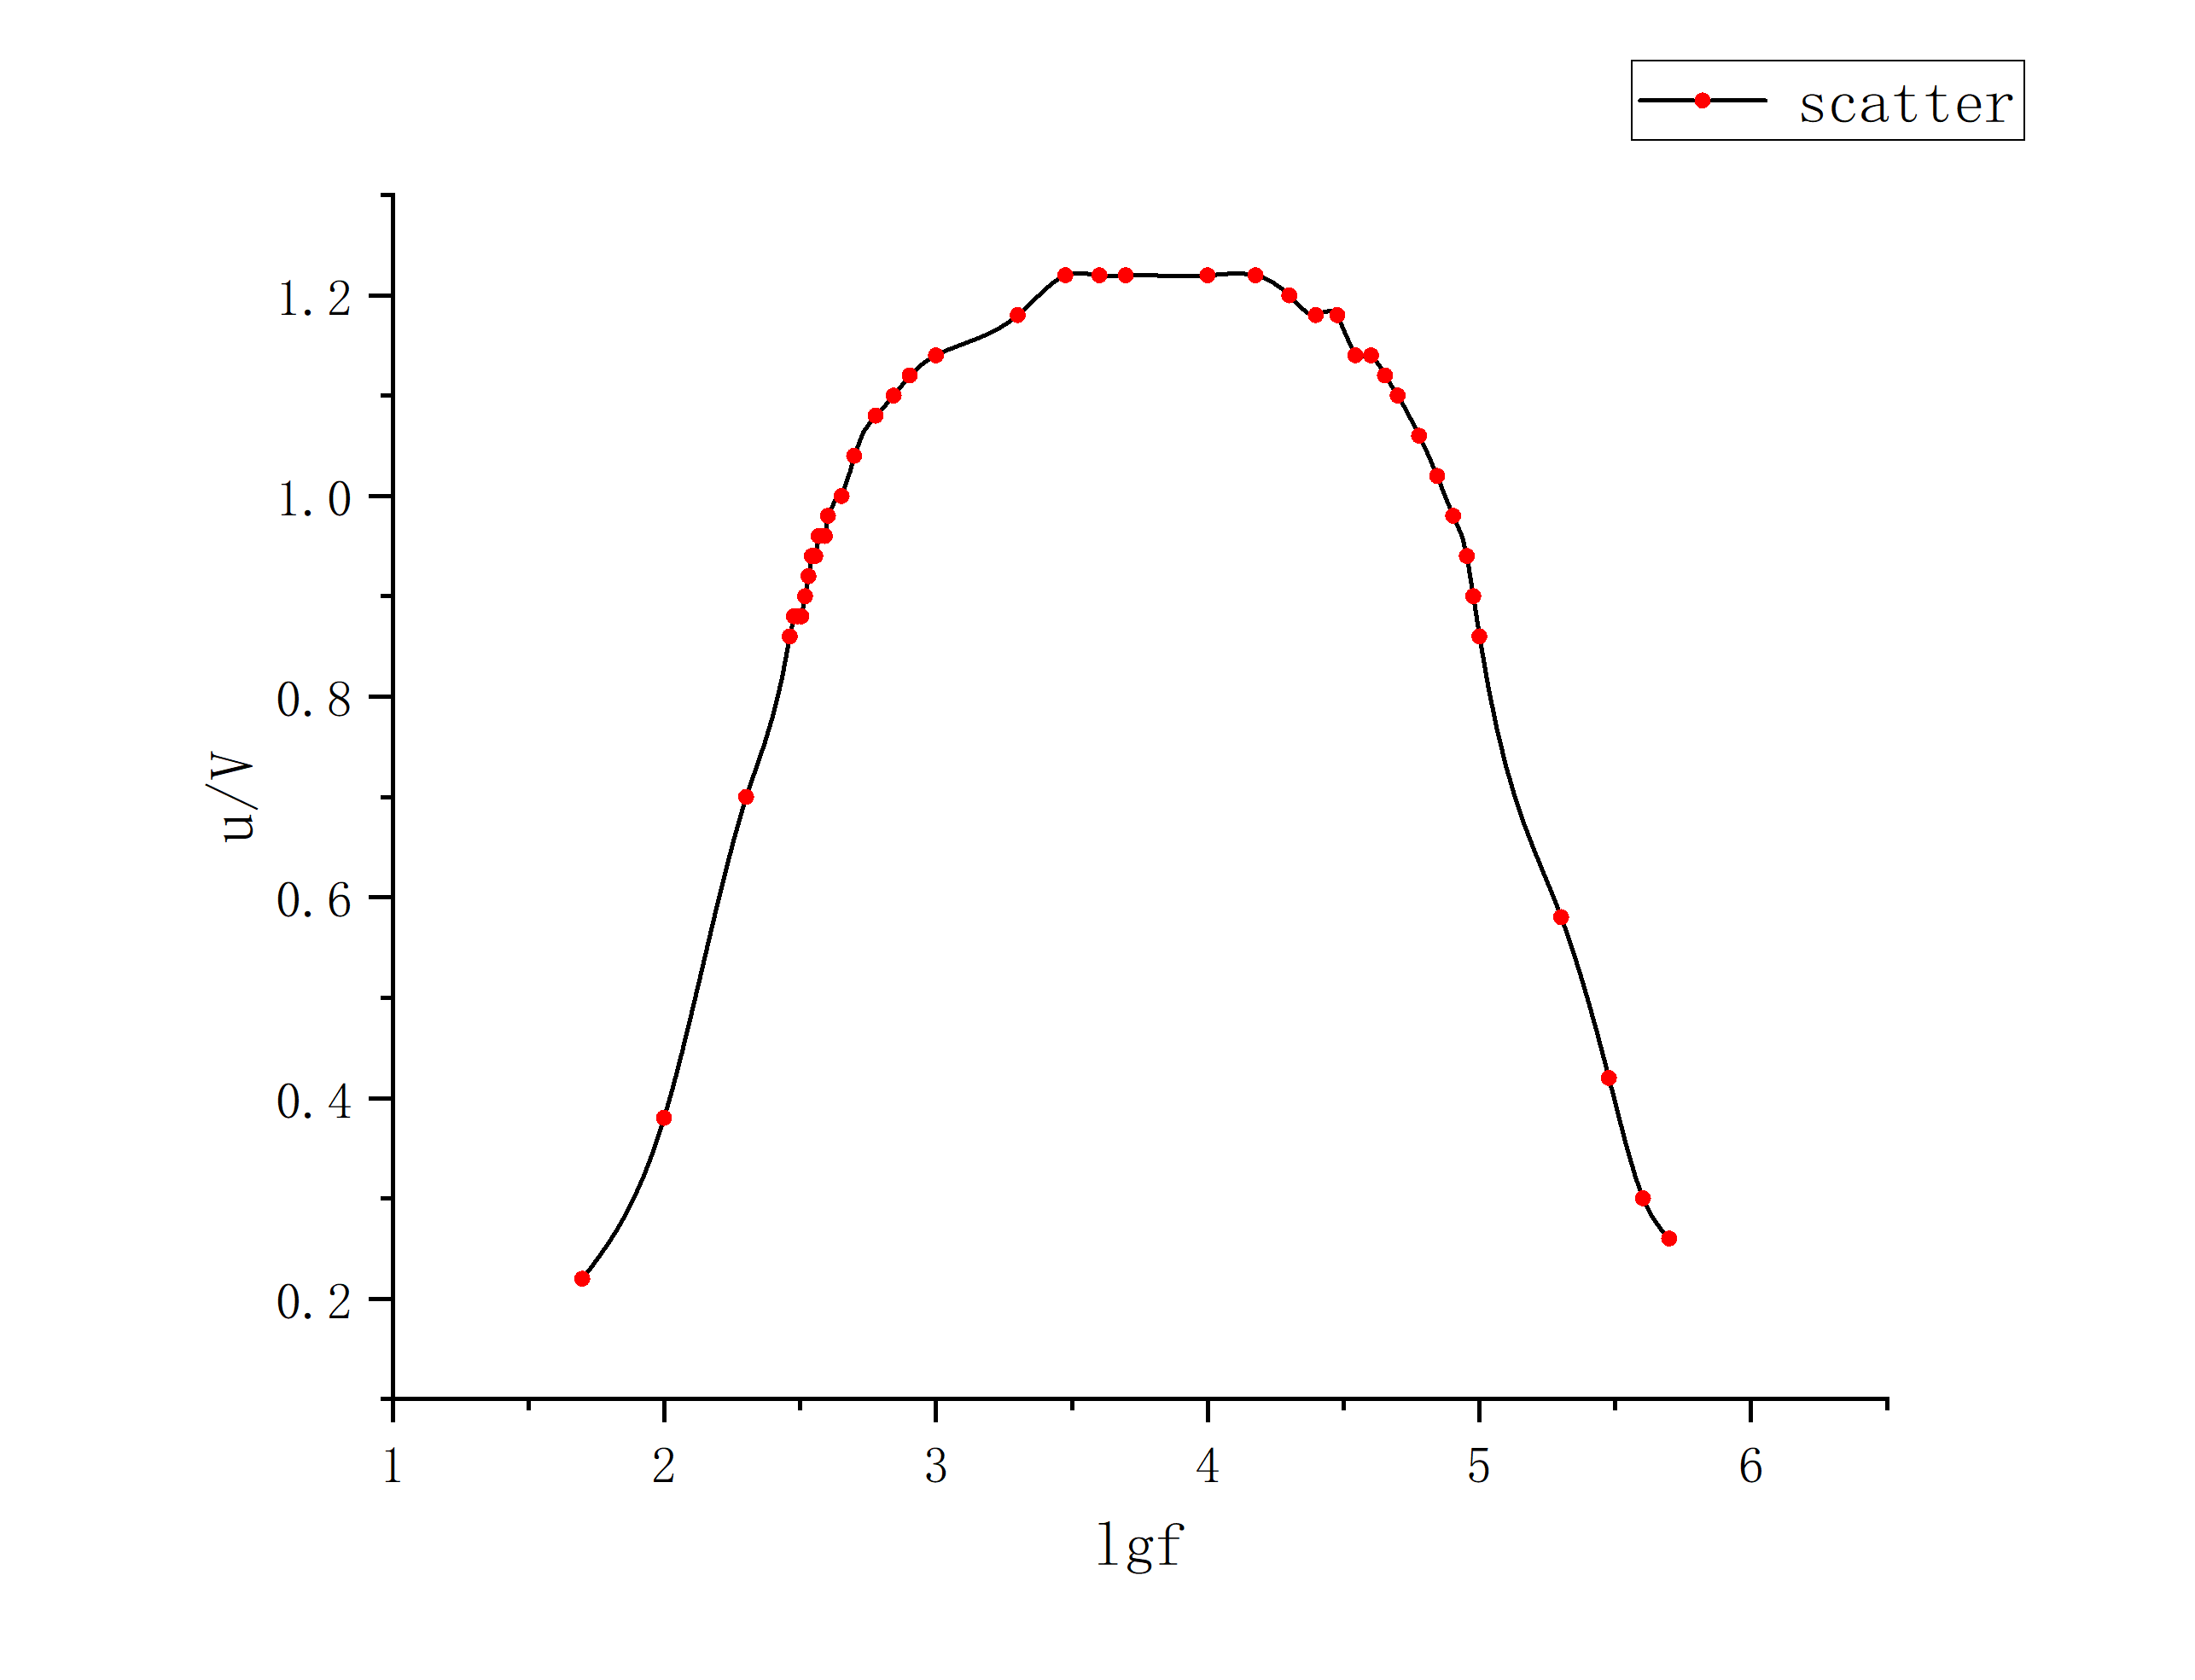
\includegraphics[width=8.8cm,height=6cm]  {实验一.png} 
	\caption{\label{1} 实验一数据图}
\end{figure}
    \subsection{开关$K_{4}$合向“0”位置}
        \begin{table}[H]
    	\centering
    	\caption{实验二数据表($u_{i}=0.252V$)}
    	\label{实验二数据表}
    	\begin{tabular}{|r|r|r|r|r|r|r|r|r|r|r|r|}
    		\toprule[0.5mm]
    		$Hz$&700&720&750&800&900&1k&1.5k&2k&3k&4k&5k\\
    		$u_{s}/V$&0.66&0.68&0.70&0.70&0.74&0.76&0.84&0.86&0.88&0.90&0.92\\
    		\bottomrule[0.5mm]
    	\end{tabular}
    \end{table}
    \par 我们可以从上表得出$f_{L}=700Hz,A_{2}\approx 3.65$。
    		\begin{figure}[H]
    	\centering
    	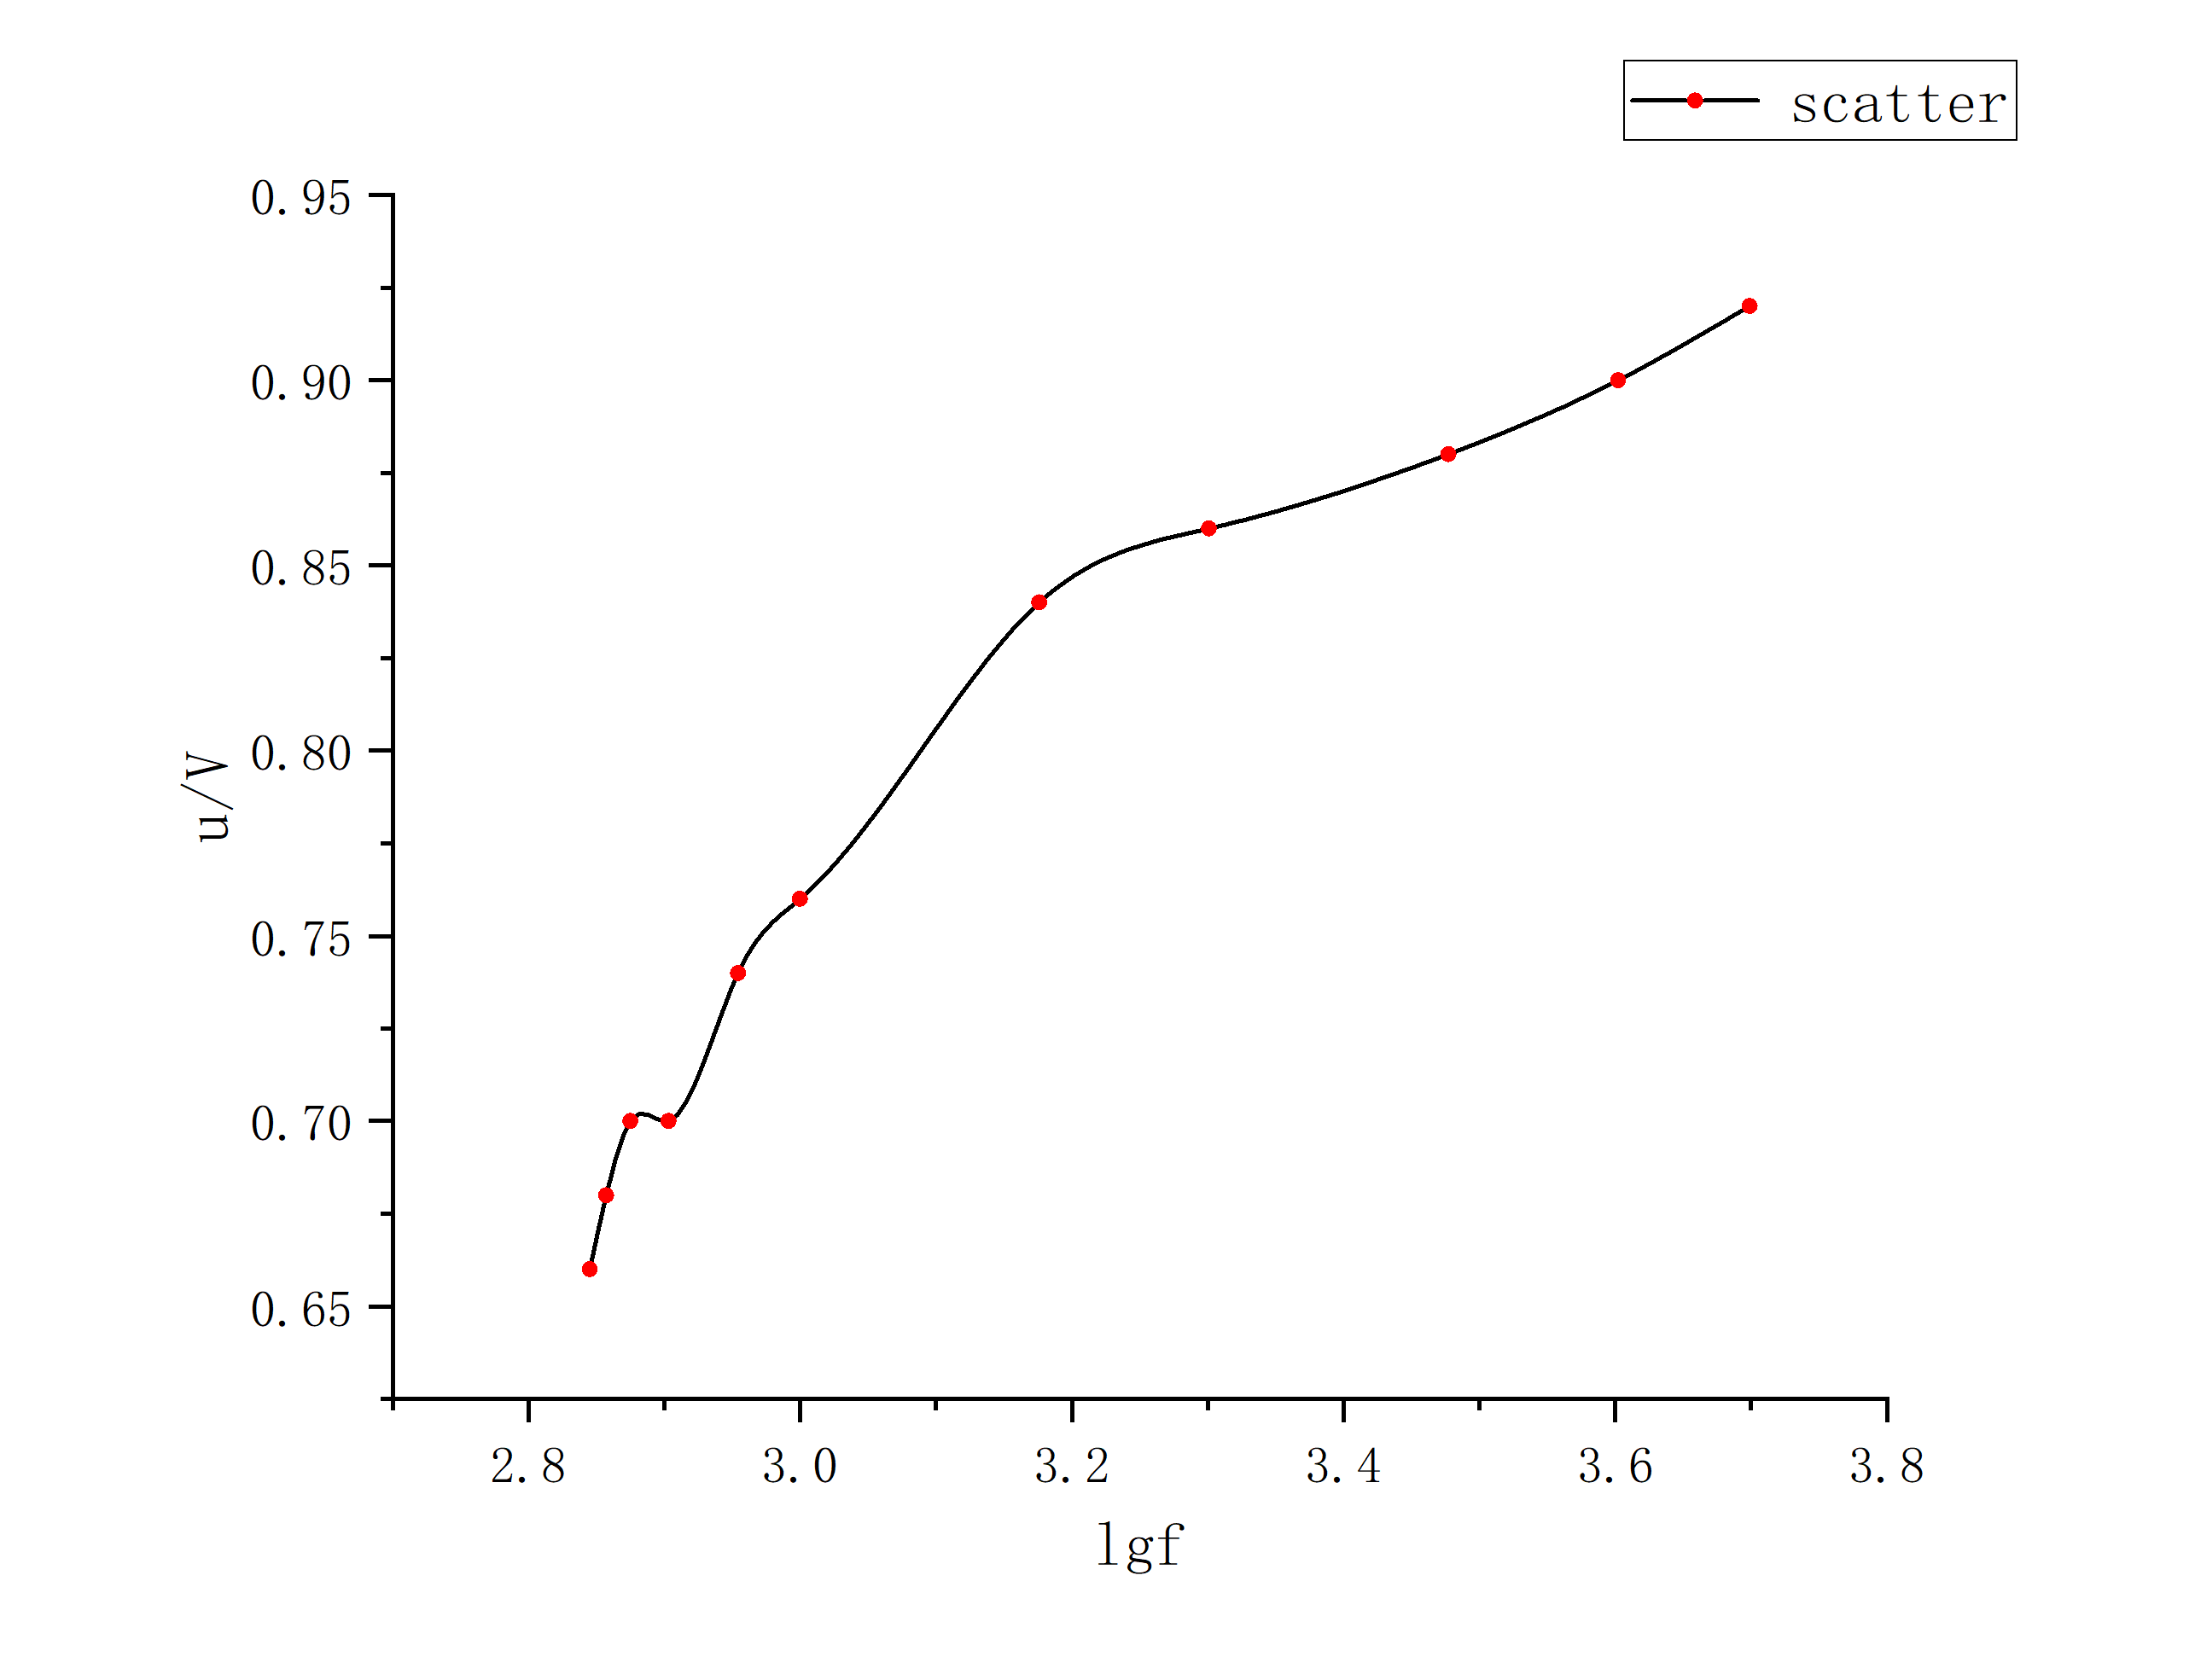
\includegraphics[width=8.8cm,height=6cm]  {实验二.png} 
    	\caption{\label{1} 实验二数据图}
    	\end{figure}
    \subsection{开关$K_{5}$合向“0”位置}
          \begin{table}[H]
    	\centering
    	\caption{实验三数据表($u_{i}=0.252V$)}
    	\label{实验三数据表}
    	\begin{tabular}{|r|r|r|r|r|r|r|r|r|}
    		\toprule[0.5mm]
    		$Hz$&85&88&90&100&200&300&400&500\\
    		$u_{s}/V$&0.92&0.94&0.98&1.04&1.22&1.26&1.26&1.28\\
    		\midrule
    		$Hz$&600&700&800&1k&2k&3k&4k&5k\\
    		$u_{s}/V$&1.28&1.28&1.28&1.30&1.30&1.30&1.30&1.30\\
    		\bottomrule[0.5mm]
    	\end{tabular}
    \end{table}
    \par 我们可以从上表得出$f_{L}=85Hz,A_{2}\approx 5.16$。
    		\begin{figure}[H]
    	\centering
    	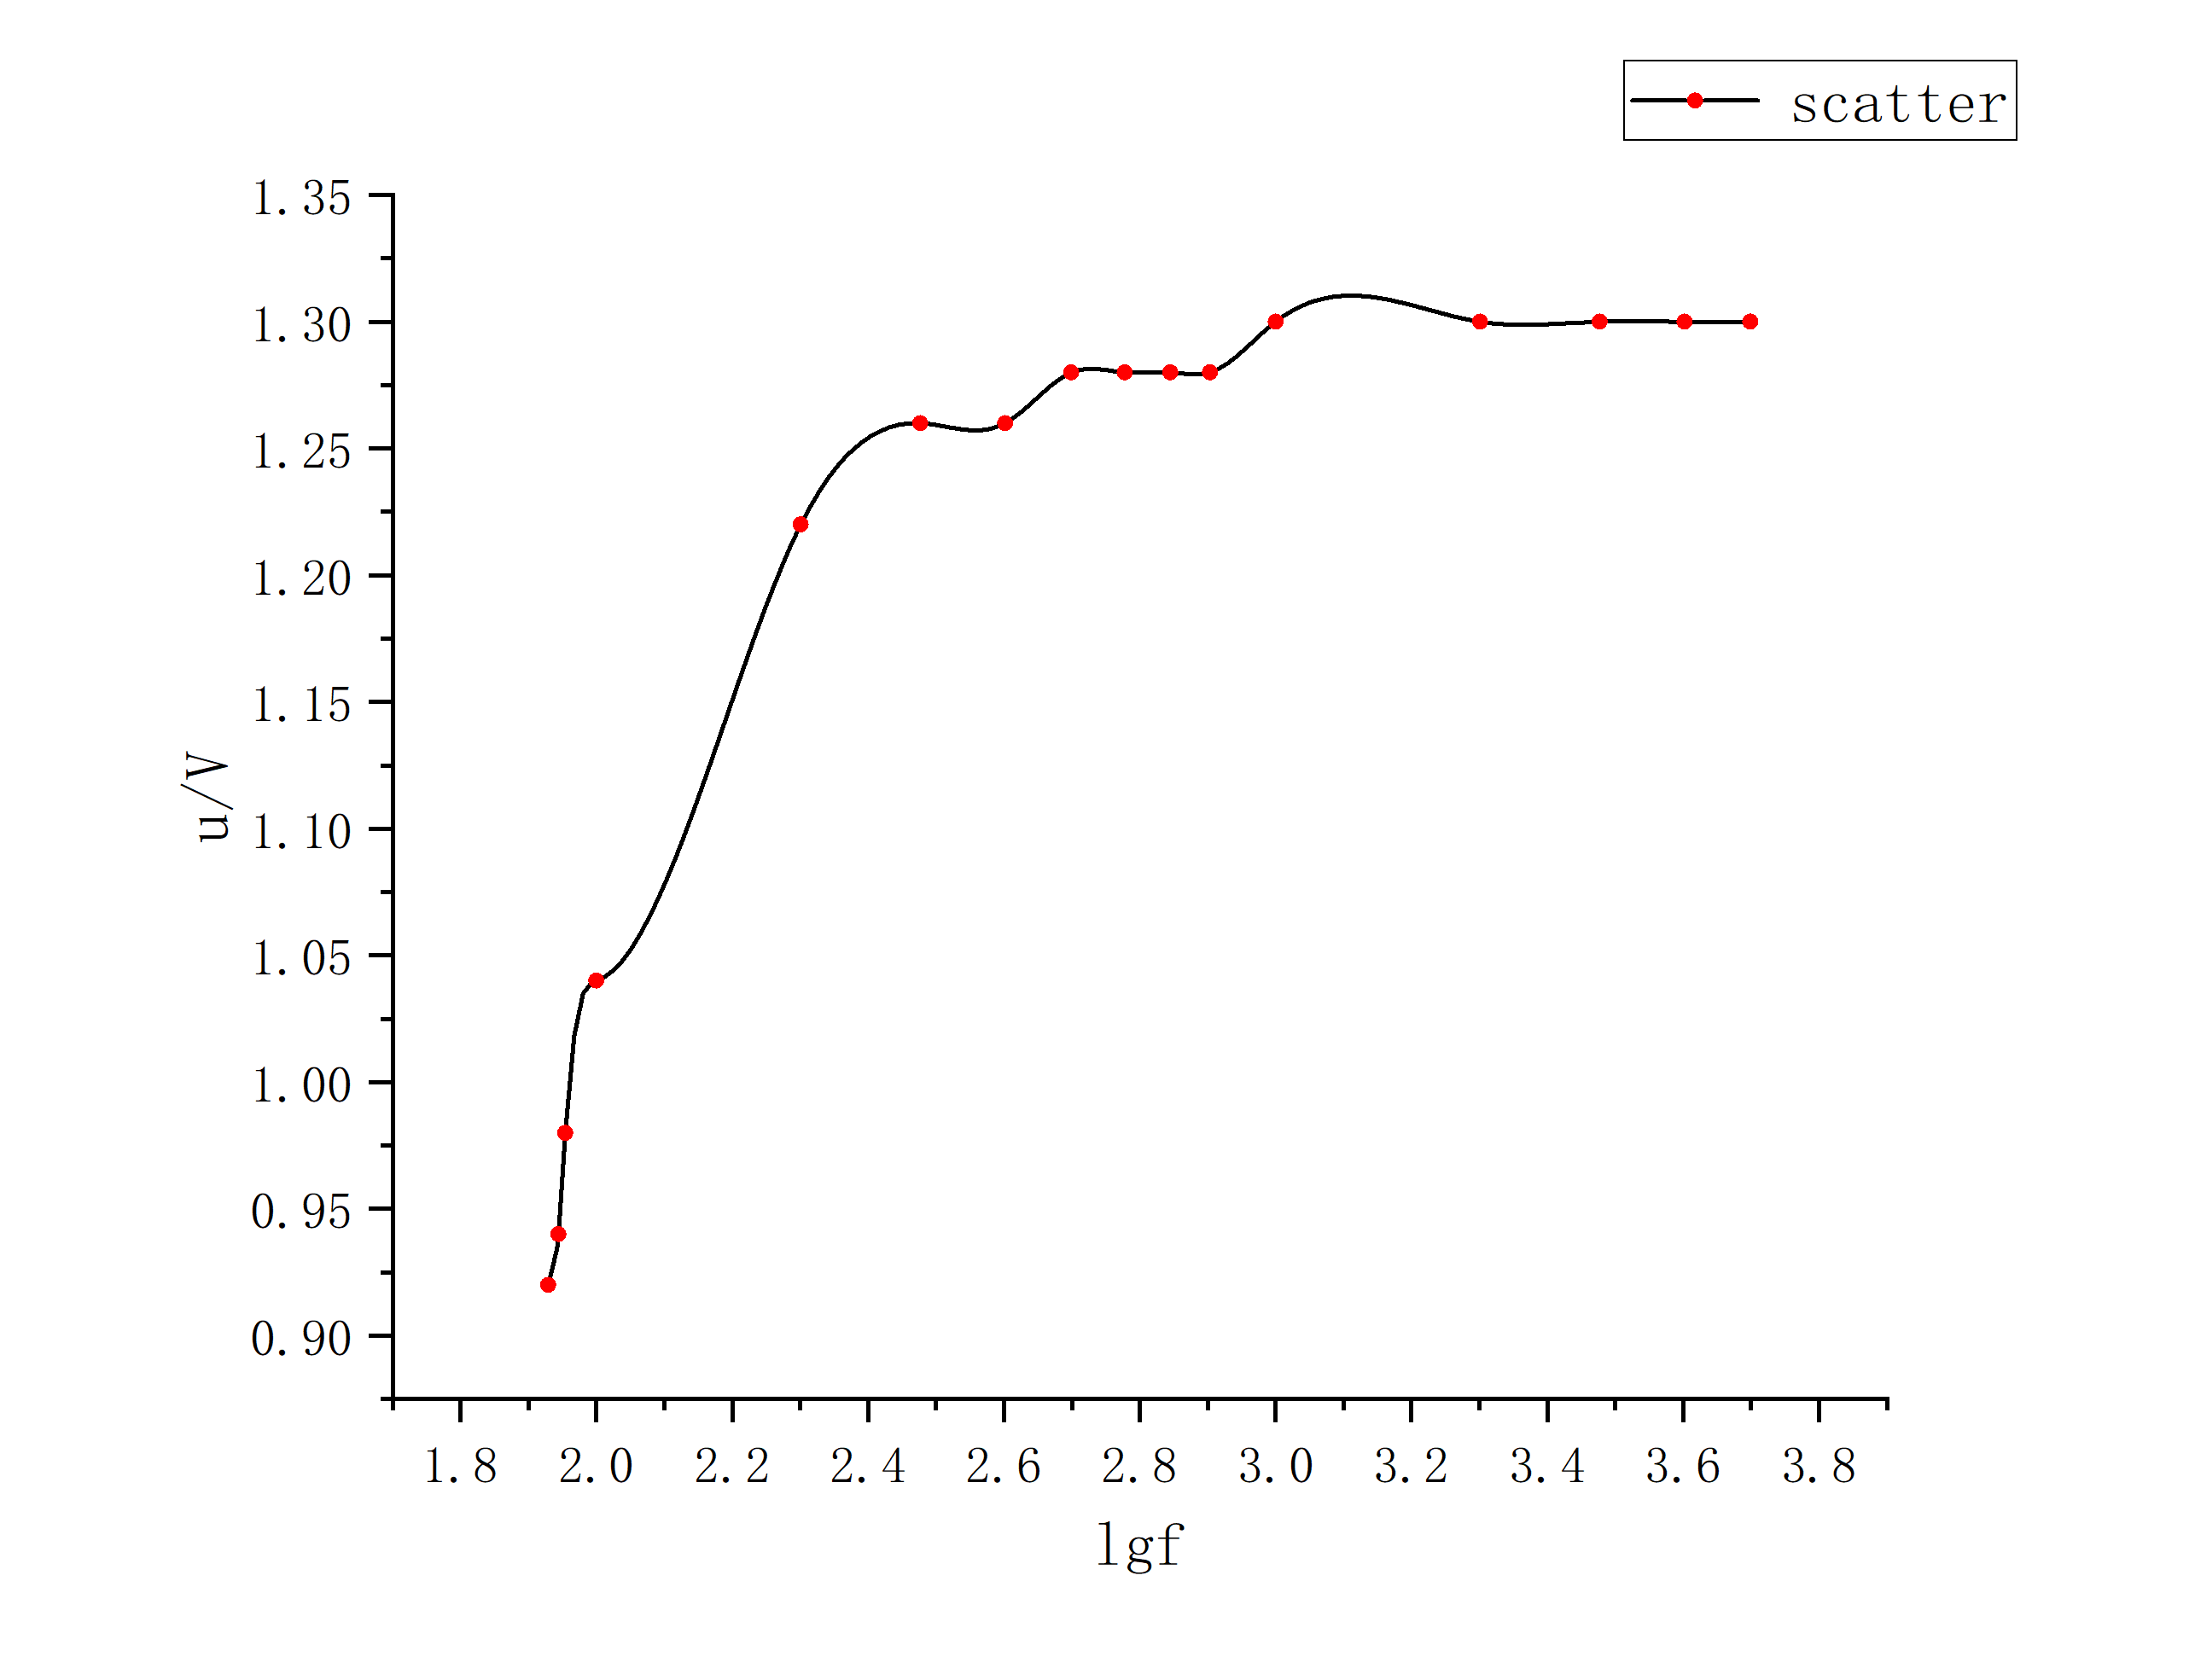
\includegraphics[width=8.8cm,height=6cm]  {实验三.png} 
    	\caption{\label{1} 实验三数据图}
    \end{figure}
    \subsection{开关$K_{6}$合向“0”位置}
              \begin{table}[H]
    	\centering
    	\caption{实验四数据表($u_{i}=0.252V$)}
    	\label{实验四数据表}
    	\begin{tabular}{|r|r|r|r|r|r|r|r|r|r|}
    		\toprule[0.5mm]
    		$Hz$&300&310&320&340&360&380&390&400&500\\
    		$u_{s}/V$&0.60&0.61&0.62&0.64&0.66&0.70&0.704&0.72&0.76\\
    		\midrule
    		$Hz$&600&700&800&900&1k&2k&3k&4k&5k\\
    		$u_{s}/V$&0.76&0.78&0.80&0.80&0.82&0.84&0.84&0.84&0.84\\
    		\bottomrule[0.5mm]
    	\end{tabular}
    \end{table}
    \par 我们可以从上表得出$f_{L}=300Hz,A_{2}\approx 3.33$。
    		\begin{figure}[H]
    	\centering
    	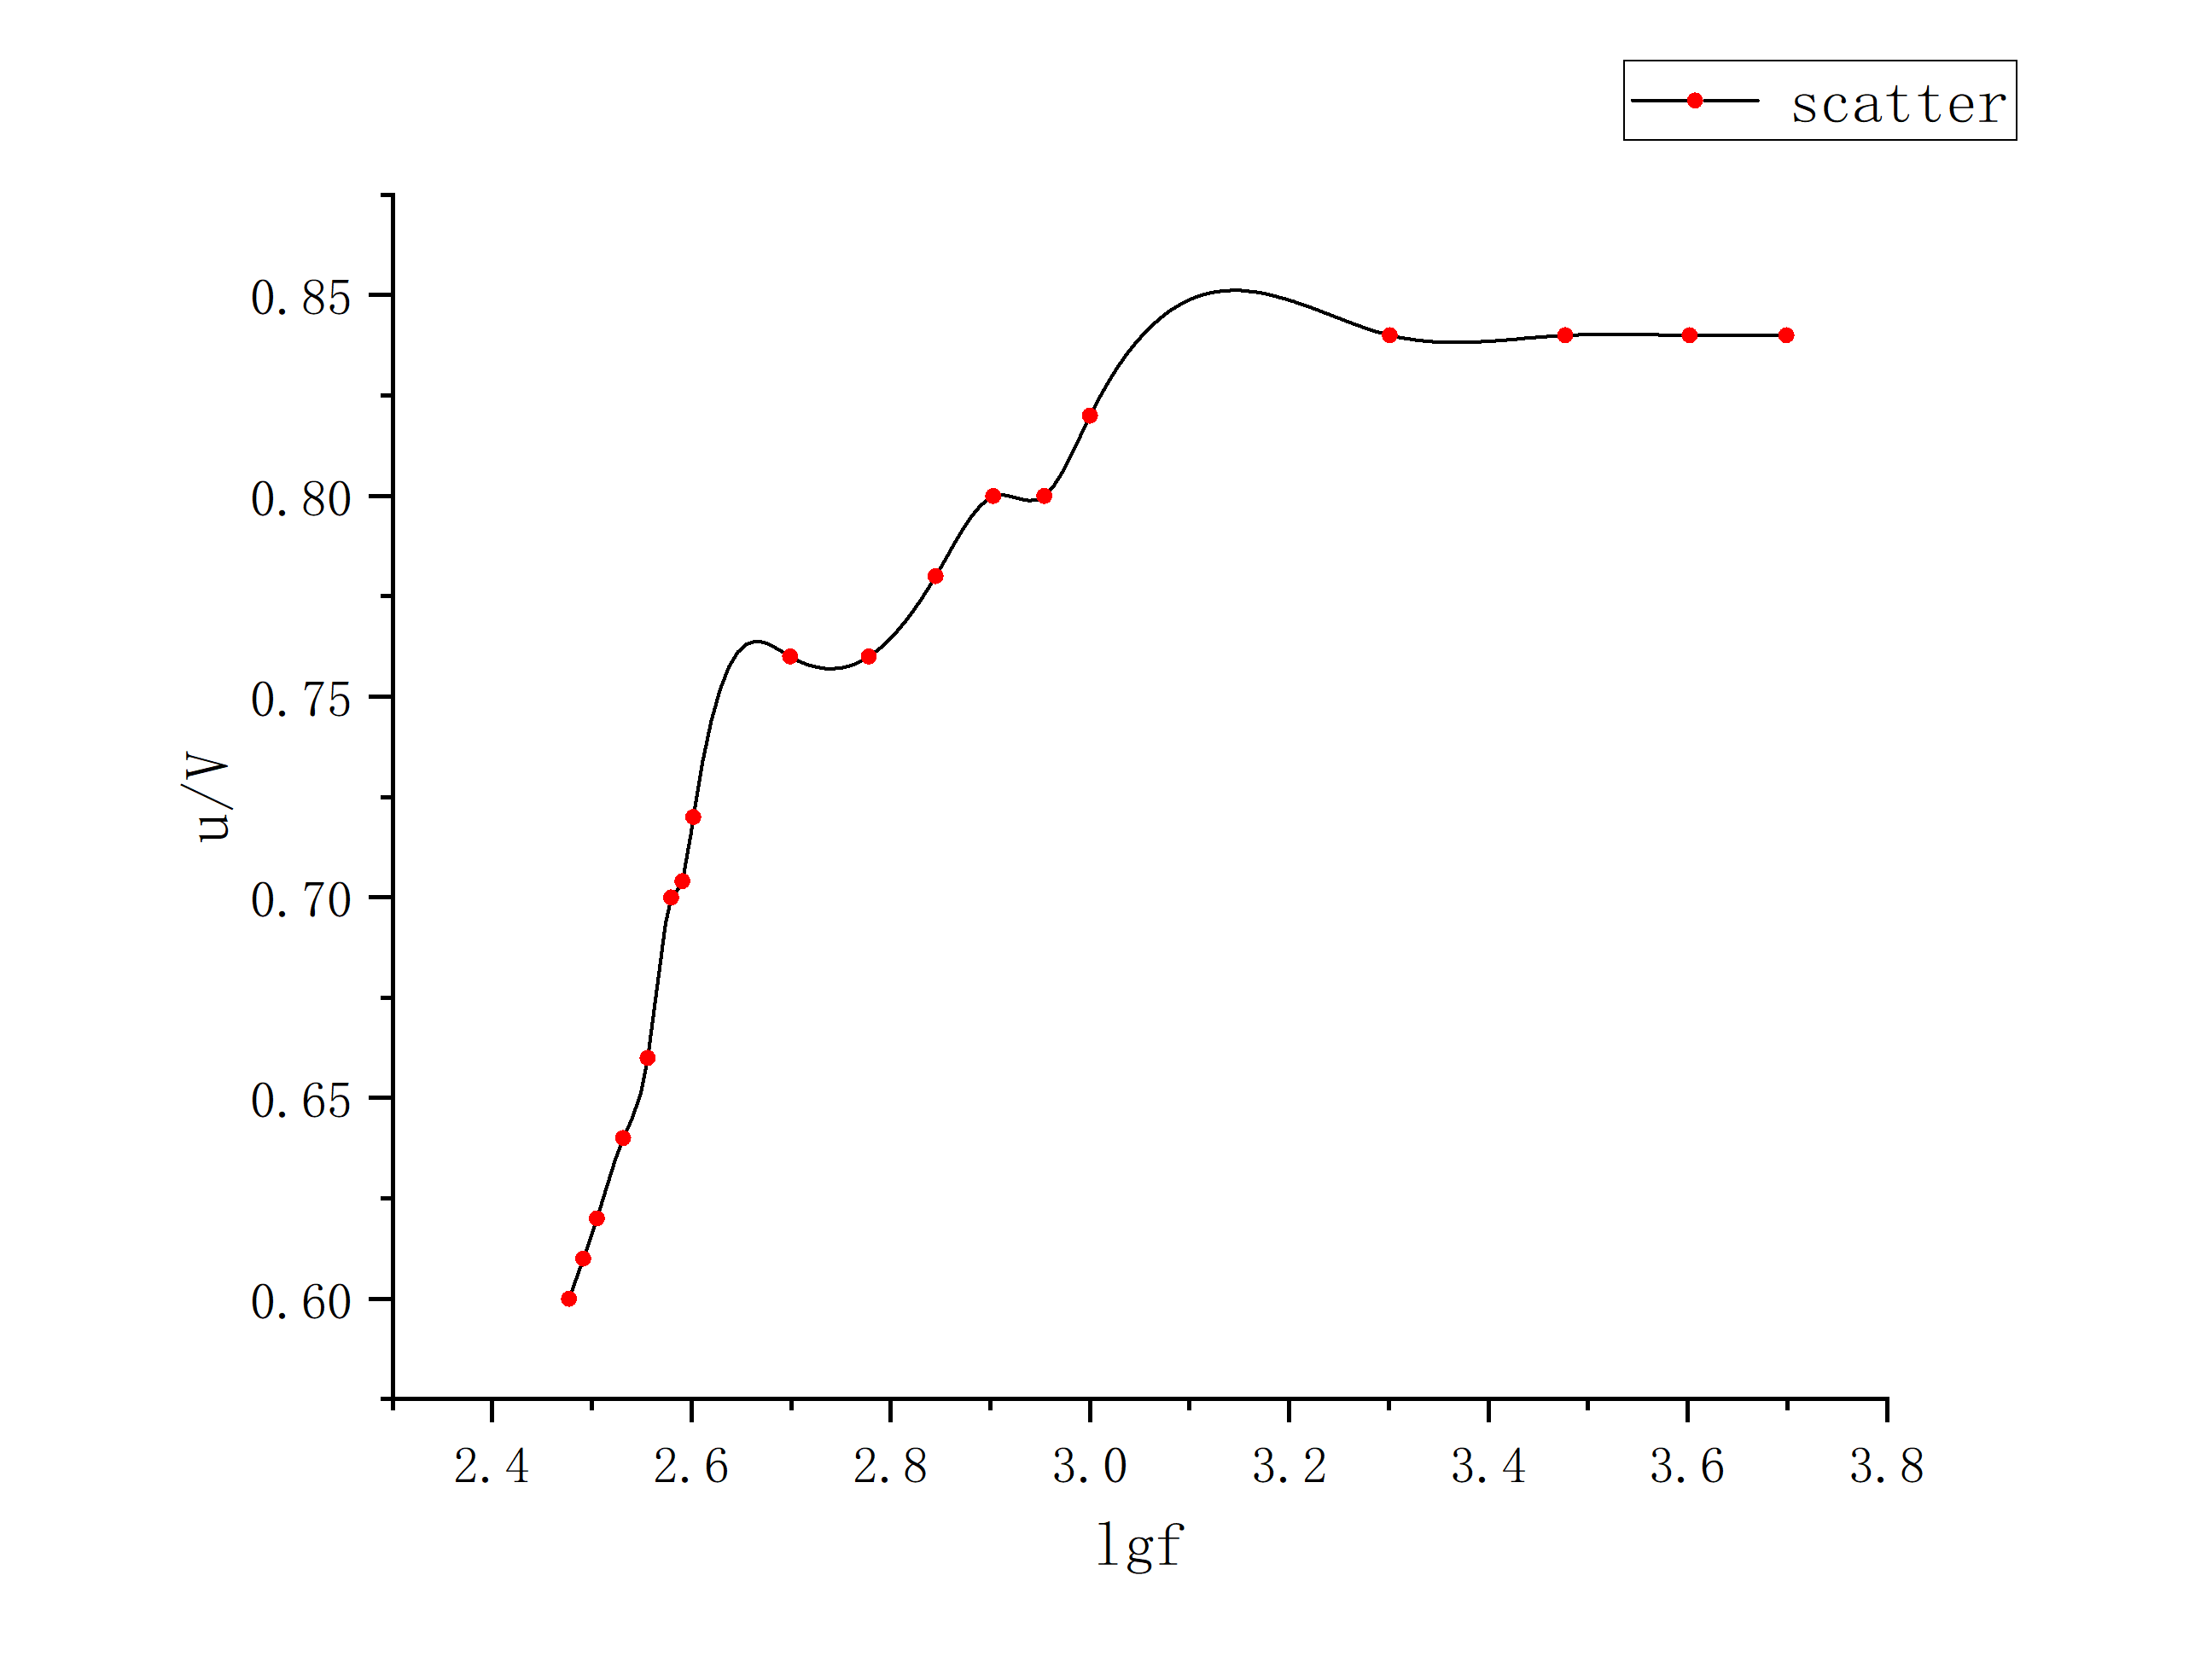
\includegraphics[width=8.8cm,height=6cm]  {实验四.png} 
    	\caption{\label{1} 实验四数据图}
    \end{figure}
    \subsection{开关$K_{7}$合向“0”位置}
                 \begin{table}[H]
    	\centering
    	\caption{实验五数据表($u_{i}=0.252V$)}
    	\label{实验五数据表}
    	\begin{tabular}{|r|r|r|r|r|r|r|r|r|r|r|}
    		\toprule[0.5mm]
    		$kHz$&5&10&20&30&40&50&60&70&80&85\\
    		$u_{s}/V$&1.12&1.10&1.10&1.06&1.02&0.96&0.92&0.88&0.82&0.80\\
    		\bottomrule[0.5mm]
    	\end{tabular}
    \end{table}
    \par 我们可以从上表得出$f_{H}=85kHz,A_{2}\approx 4.44$。
    		\begin{figure}[H]
    	\centering
    	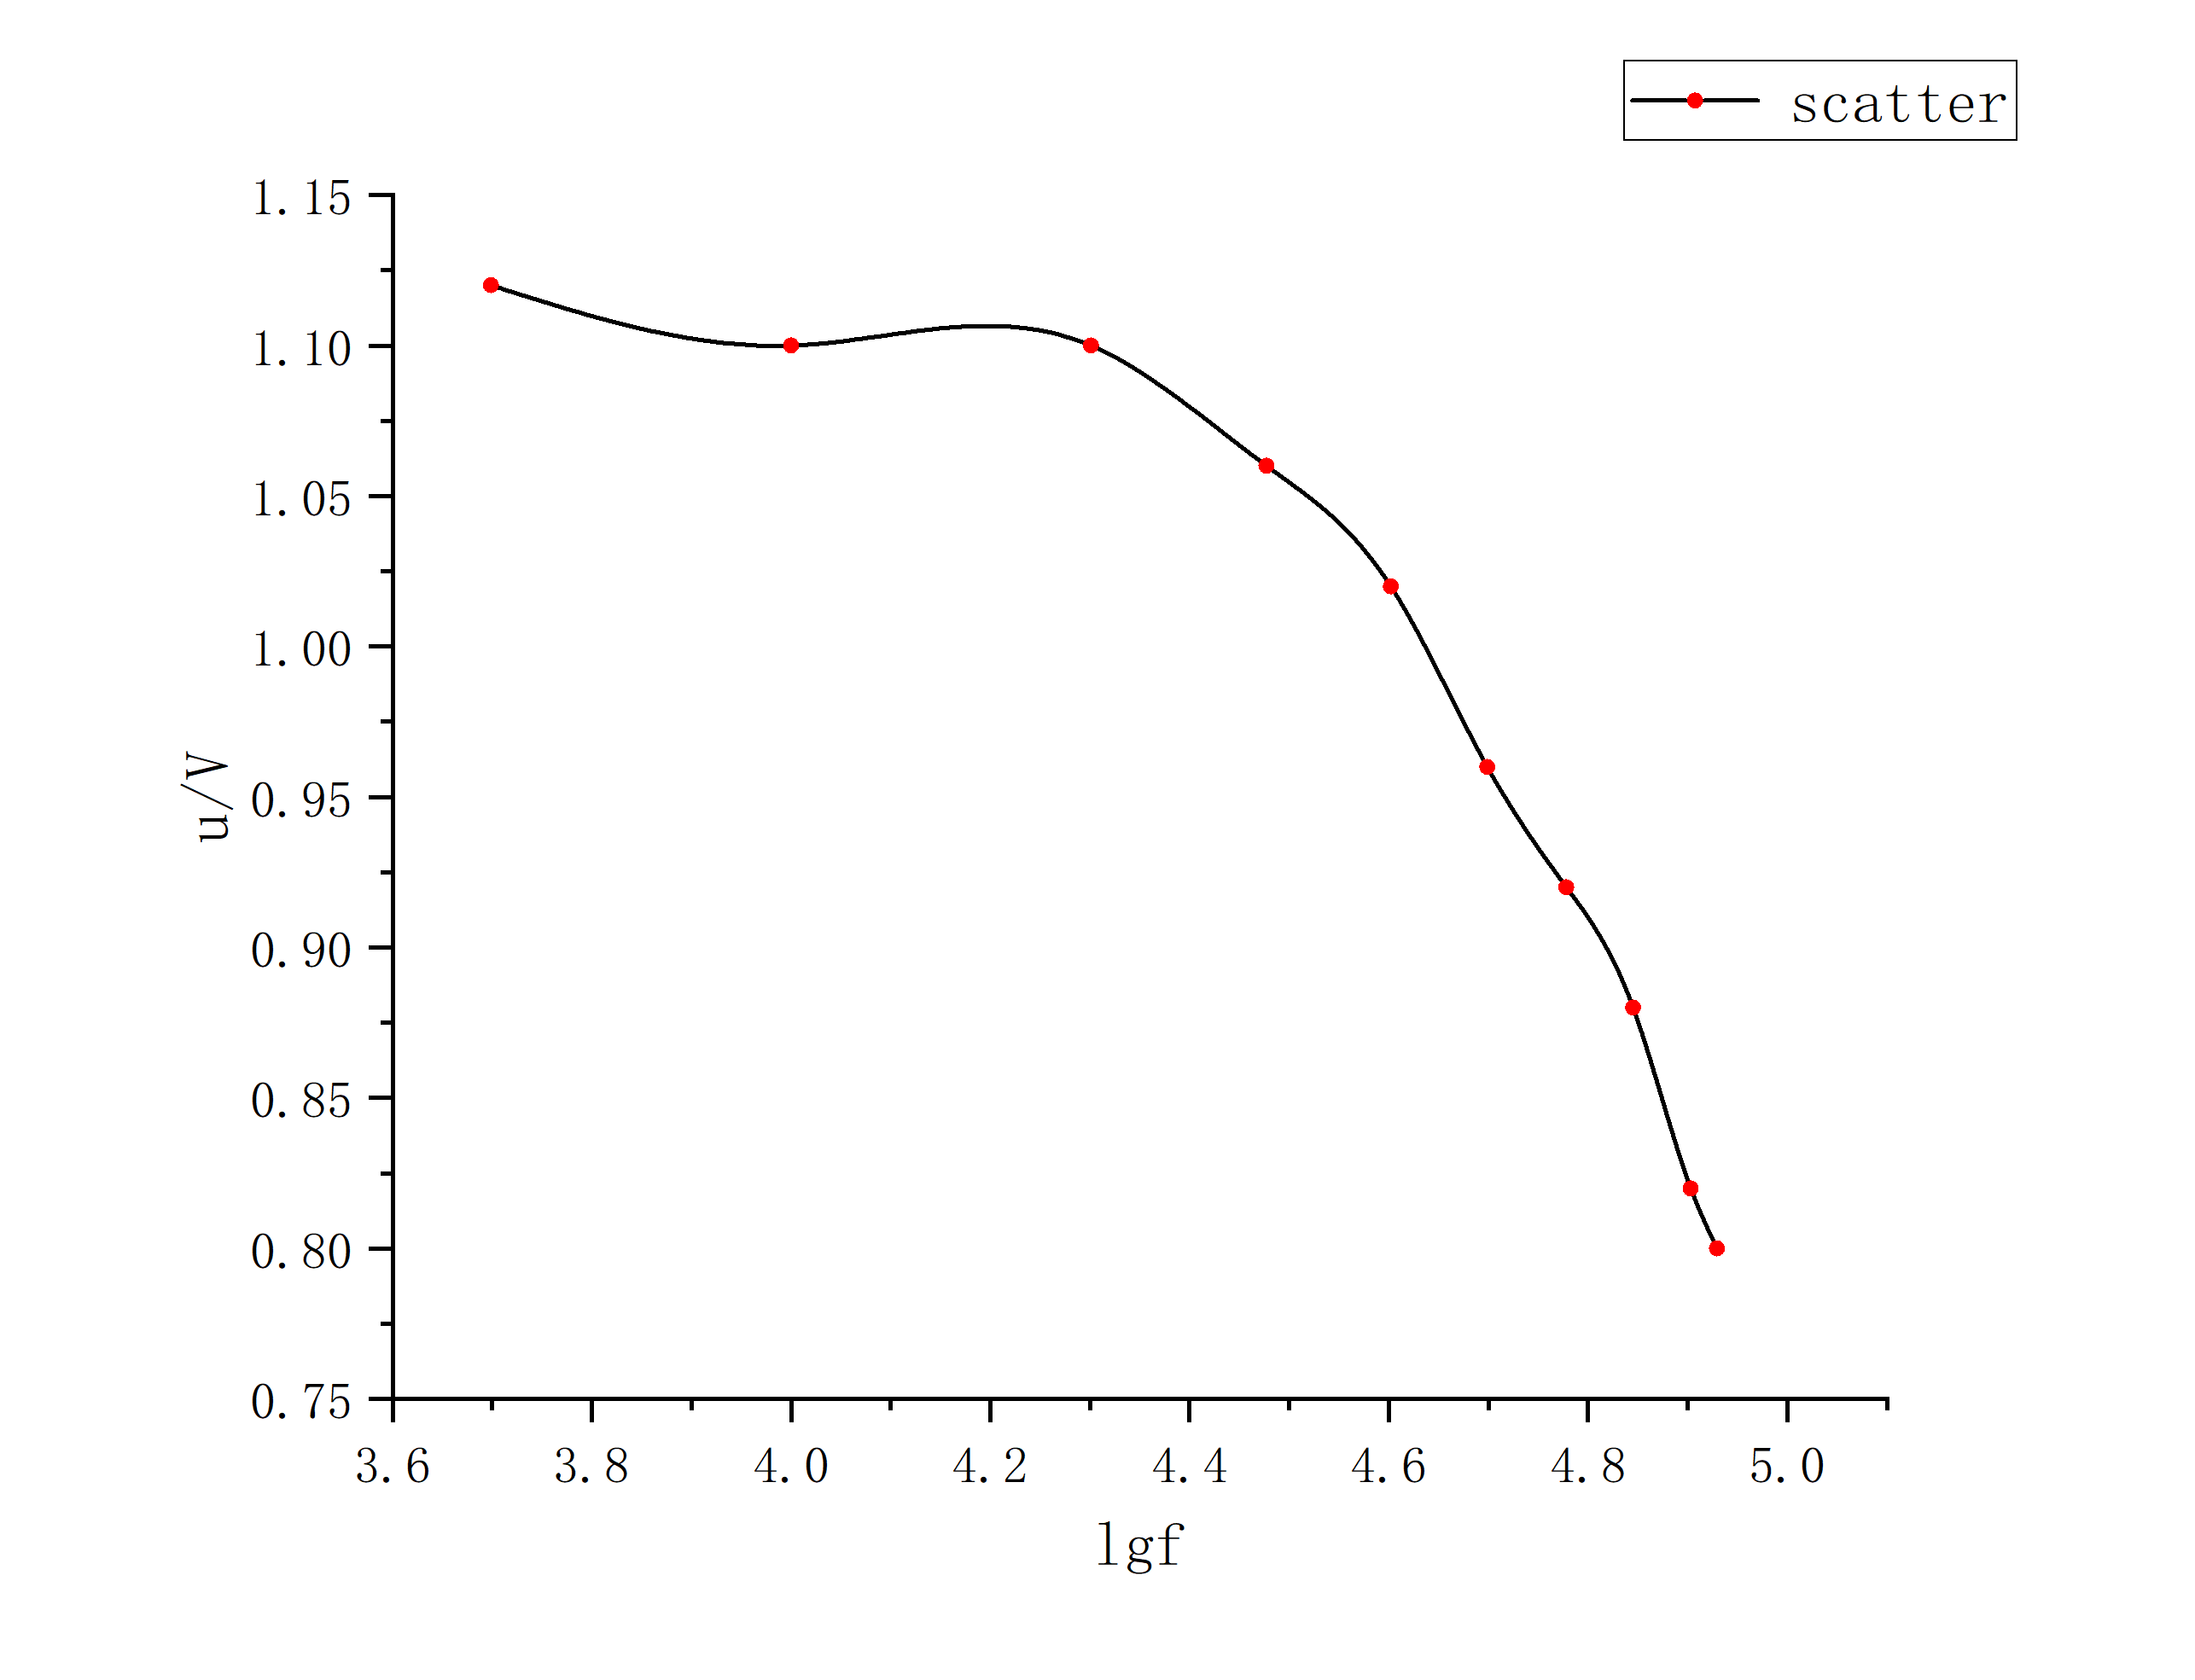
\includegraphics[width=8.8cm,height=6cm]  {实验五.png} 
    	\caption{\label{1} 实验五数据图}
    \end{figure}
    \section{思考题}
    \small{(1)为什么测量放大器频率响应所用的示波器或毫伏表都须有足够的频宽?如果被测放大器的频带比所用毫伏表或示波器的频带宽,将出现什么问题?
    \par 答:因为如果示波器或者毫伏表的频宽不够,则在低频或者高频处测得的输出信号将会由于低频或高频信号丢失而失真;如果被测放大器的频带比所用毫伏表或示波器的频带宽,将会出现测得输出信号电压值不准,而无法准确得到电路的上限或者下限频率。
    \par (2)用描点法测量放大器的频率响应曲线,有哪些步骤与注意点?为什么要保持放大器的输入信号幅度不变?能不能保持输出电压不变?如果能,怎样测量?
     \par 答:先用$200mV_{p-p}$,5kHz的信号试探,然后监视输入信号不变,改变频率同时记录输出信号强度的变化,在输出电压变化缓慢部分少测点,在变化迅速的部分多测点,使用示波器多次平均的功能;因为若不保持输入信号幅度不变,则不能保持单一变量,数据之间不能进行比较;能,在保持图形不失真的情况下,保持输出电压不变,改变输入电压,则输入电压变为初始时的$\sqrt{2}$倍时的频率为上限或下限频率。
    \par (3)什么叫通频带,它是如何定义的?怎样求出频带的高低频截止频率 $f_{H}$、$f_{L}$?如果不测频率响应曲线,能不能直接测出通频带的高低截止频率?
     \par 答:通频带为电路上限与下限截止频率之间的范围;在一个较宽范围内放大倍数一致,减小频率使得放大倍数变为原来的$\frac{1}{\sqrt{2}}$时的频率为低频截止频率,增加频率使得放大倍数变为原来的$\frac{1}{\sqrt{2}}$时的频率为高频截止频率;可以通过测量电路每个电容的开路时间常数和的倒数求得上限截止频率,测量每个电容的短路时间常数和的倒数来求得下限截止频率。
    \par (4)级联后各级放大器静态工作点有无变化?为什么?
     \par 答:无变化,因为此为阻容耦合级联,由于电容的隔绝直流的作用,所以各级放大器的静态工作点不变。}
\begin{appendices}
	\section{原始数据整理}
		\begin{figure}[H]
		\centering
		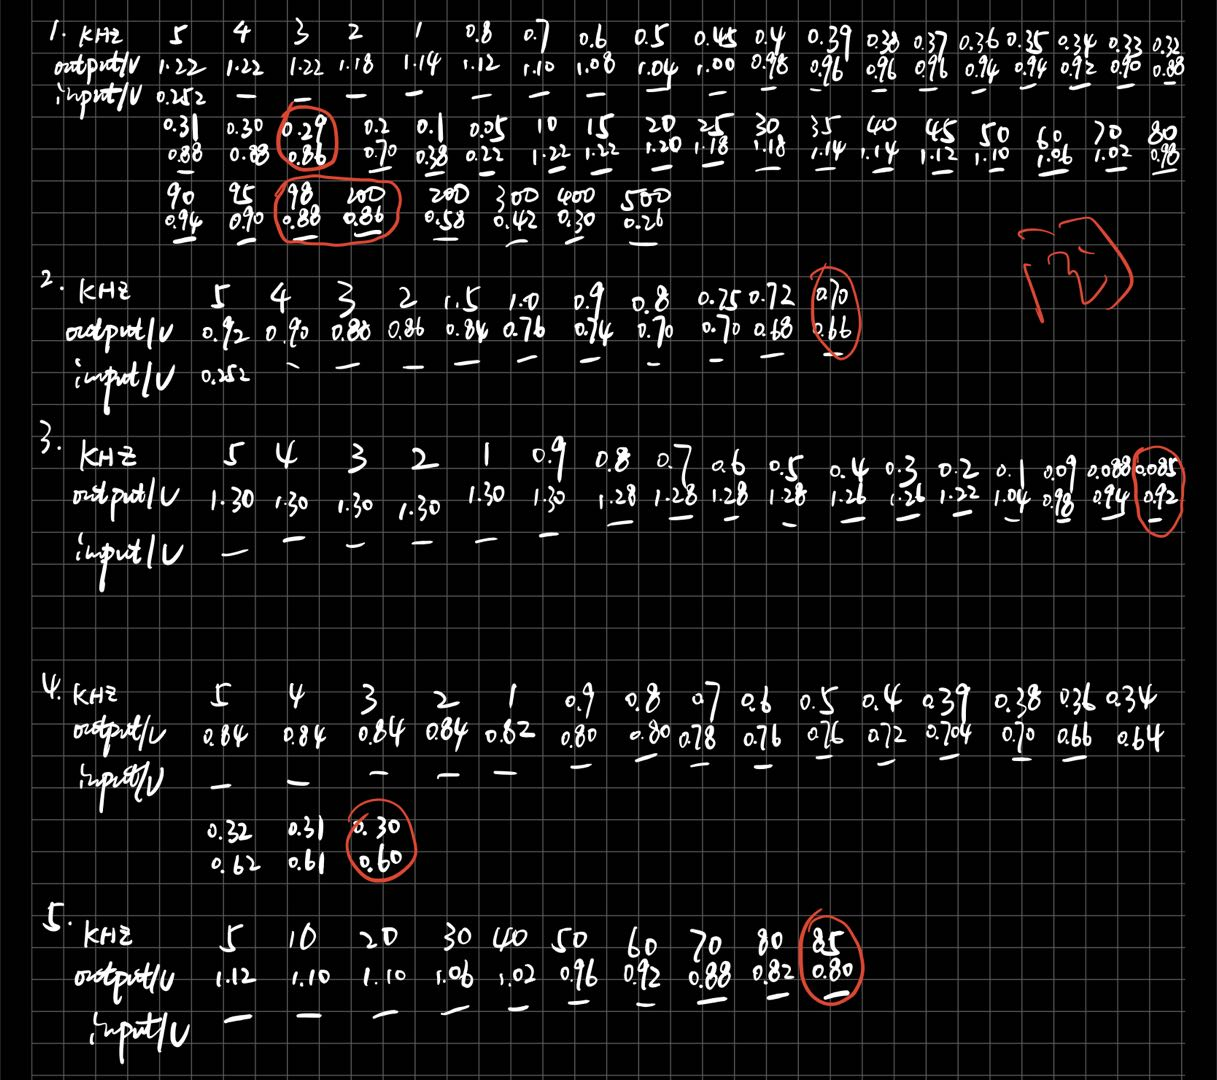
\includegraphics[width=11.1cm,height=9cm]  {放大器.jpg} 
		\caption{\label{1} 原始数据截图}
	\end{figure}
\end{appendices}
\end{document} 
